\documentclass[a4paper,12pt, oneside]{book}
\usepackage[swedish]{babel} % choose the language
\usepackage[utf8]{inputenc} % äöå
\usepackage[T1]{fontenc}
\usepackage[a4paper, inner=3cm, outer=3cm, top=3cm, bottom=3cm]{geometry}
\usepackage{mathptmx} % Times New Roman
\usepackage{tikz} % Support for pictures in latex format -> convert svg files into tikz format at first
\usepackage{etoolbox} % this one makes a workaround with page numbering possible
\usepackage{float}

\usepackage[style=numeric-comp,sorting=none,backend=biber,language=swedish]{biblatex}

\usepackage{csquotes} % BibLaTex stuff
\usepackage[
  style=numeric-comp,
  sorting=none,
  backend=biber
]{biblatex}
\ExecuteBibliographyOptions{url=true, doi=true}
\addbibresource{Kapitel/referenser.bib}

\usepackage[
  colorlinks=true,
  linkcolor=black,
  citecolor=black,
  urlcolor=blue
]{hyperref}
\usepackage{xurl}

\usepackage{setspace}

% Table of contents
\setcounter{secnumdepth}{5}
\setcounter{tocdepth}{5}

%------------Titel-----------%
\begin{document}

\pagestyle{empty}    
\begingroup
\patchcmd{\chapter}{plain}{empty}{}{}

\begin{titlepage}
    \newgeometry{left=2.5cm,right=2.5cm,top=2.5cm,bottom=2.5cm}
    \thispagestyle{empty}

    \begin{flushleft} 
        \includegraphics[width=2.5cm]{Bilder/ÅA logo}
    \end{flushleft}   
    
    \vspace*{0.5cm}
    
    \begin{center}
        {\huge \textbf{Social engineering inom cybersäkerhet}}\\[0.6cm]
        {\Large Psykologiska och tekniska aspekter av digital manipulation}\\[0.6cm]

    \vfill
    \begin{center}
        \includegraphics[width=6.5cm, height=6.5cm]{Bilder/ÅA signum}
    \end{center}
        
    \end{center}

    \vfill

    \hfill
    \begin{flushright}
        Max Ruotsalainen\\
        Kandidatavhandling i datateknik\\
        Handledare: Annamari Soini\\
        Fakulteten för naturvetenskap och teknik\\
        Åbo Akademi\\
        2026
    \end{flushright}
    \restoregeometry
\end{titlepage}

\clearpage
\pagestyle{plain}    
\onehalfspacing
\section*{\LARGE Referat}
\thispagestyle{empty}

I ett växande samhälle där digitala tjänster, molnplattformar och nätverksbaserade system kontinuerligt integreras i både offentliga och privata verksamheter, ökar betydelsen av cybersäkerhet. I takt med att skyddsåtgärder utvecklas förändras hotbilden. En särskilt framträdande kategori av hot är social engineering, där hotaktörer inte direkt utnyttjar tekniska sårbarheter utan manipulerar mänskligt beteende och beslutsfattande. Avhandlingen analyserar social engineering som ett cybersäkerhetshot i moderna digitala miljöer med fokus på hur tekniska verktyg och psykologiska mekanismer samverkar för att möjliggöra framgångsrika cyberattacker.

Utvecklingen av artificiell intelligens och generativa modeller har ytterligare förändrat hotlandskapet. Djupfejkteknik och AI-genererat innehåll skapar nya möjligheter för hotaktörer att producera mer trovärdiga och tekniskt sofistikerade bedrägerier. Även om hotbilden har ökat i komplexitet, finns det olika tekniska och organisatoriska försvarsmekanismer som kan användas för att minska risken för manipulation. Genom att förstå social engineering som ett sociotekniskt säkerhetshot, där tekniska, organisatoriska och mänskliga faktorer samverkar, kan mer effektiva skyddsåtgärder utvecklas.

\section*{\LARGE Nyckelord}
Social engineering, socio-tekniskt fenomen, cybersäkerhet, artificiell intelligens
%----------Innehållsförteckning------------%
\tableofcontents 

\endgroup % end of TeX group

\clearpage
\pagestyle{plain}    

\onehalfspacing

\pagenumbering{arabic} % Page numbering starts from here

\chapter{Inledning}
Traditionellt har cybersäkerhet främst fokuserat på tekniska skyddsmekanismer, som brandväggar, kryptering och intrångsdetektion, men med digitaliseringens raska framsteg och förekomsten av nya angreppsmetoder har skyddet mot dessa hot blivit allt mer komplicerat \cite{cybersakerhet_kommuner}. Enligt \cite{heartfield_loukas_se, algarni2019se_survey} har hotaktörer börjat i allt större grad utnyttja mänskliga faktorer snarare än enbart tekniska sårbarheter. Social engineering definieras därmed som en angreppsform där psykologisk manipulation används för att få individer att lämna ut känslig information eller utföra handlingar som äventyrar säkerheten \cite{psychology_social_engineering}. Därför bör social engineering förstås som ett socio-tekniskt fenomen där tekniska system, organisatoriska strukturer och mänskligt beslutsfattande används för att begå brott \cite{washo2021interdisciplinary}.

Eftersom människan spelar en avgörande roll i social engineering-relaterade incidenter har den Europeiska unionens cybersäkerhetsbyrå (ENISA) börjat betona vikten av hur individuella beteenden, organisatoriska kulturer och arbetsprocesser påverkar förebyggandet av dessa attacker \cite{enisa2018cybersecurity_culture}. Detta innebär att endast tekniska skyddsåtgärder inte är tillräckliga för att hantera cyberhotet. Därtill har utvecklingen av artificiell intelligens (AI) ytterligare förändrat social engineering som ett cyberhot. Generativ AI har börjat användas för att producera mer avancerade attacker, vilket i sin tur har försvårat identifiering och detektion \cite{zhang2024digital_deception}. Samtidigt har AI också blivit ett verktyg för att stärka försvarssystemen genom avancerad mönsterigenkänning och hotanalys. Detta har lett till en kontinuerlig kapprustning där både hotaktörer och organisationer strävar efter att ha försprång.

\section{Syfte}
Syftet med denna kandidatavhandling är att analysera social engineering som ett cybersäkerhetshot med ett särskilt fokus på samspelet mellan tekniska och psykologiska faktorer. Avhandlingen ämnar att föra fram hur social engineering-attacker fungerar, varför de är effektiva och hur de kan förstås inom ramen för cybersäkerhetens socio-tekniska perspektiv. Som grund för avhandlingen används litteraturstudier där vetenskapliga artiklar, översiktsstudier och relevanta rapporter analyseras och sammanställs. Målet med avhandlingen är att bidra till en fördjupad förståelse av social engineering genom att identifiera centrala utmaningar kopplade till detektion och förebyggande av denna typ av cyberhot. 

\section{Forskningsfrågor}
I avhandlingen kommer fyra forskningsfrågor att behandlas. Inledningsvis förklaras social engineering i kontexten av modern cybersäkerhet. Därefter analyseras de psykologiska och tekniska mekanismer som möjliggör social engineering som ett effektivt cyberhot. Slutligen undersöks metoder som finns för att motverka, identifiera och filtrera social engineering i praktiken. Forskningsfrågorna ser ut som följande:
\begin{enumerate}
    \item Vilka psykologiska mekanismer bidrar till att social engineering-attacker är effektiva?
    \item Vilka tekniska metoder och attacktyper används i dagens social engineering-attacker?
    \item Vilka identifierings- och detektionsmetoder kan användas för att upptäcka social engineering?
    \item I vilken grad kan artificiell intelligens och automatiserade system bidra till att förebygga och motverka social engineering?
\end{enumerate}


\section{Disposition} 

\chapter{Bakgrund och teori}
Detta kapitel presenterar den teoretiska bakgrund som krävs för att förstå social engineering som ett cybersäkerhetshot. Inledningsvis diskuteras cybersäkerhetens roll i moderna digitala system och grunden för att förstå cybersäkerhet i dagens digitala miljöer. Kapitlet kommer också att behandla social engineering som ett fenomen, med fokus på dess unika angreppssätt som utnyttjar mänskliga faktorer snarare än enbart tekniska sårbarheter. Avslutningsvis diskuteras de psykologiska mekanismer som ligger till grund för social engineering-attacker och en genomgång av vanliga angreppsmetoder och attacktyper.

\section{Cybersäkerhet i moderna digitala system}
Under de senaste årtiondena har digitaliseringen lett till att samhällsfunktioner, organisationer och individer blivit alltmer beroende av digitala system. Utvecklingen har möjliggjort effektivare verksamhetsprocesser och skapat ett överflöd av nya digitala tjänster. Däremot har utvecklingen också samtidigt ökat systemens exponering för cyberhot och expanderat attackytan för hotaktörer \cite{gururaj2024social_engineering}.

För moderna digitala system kan cybersäkerhet förstås som skyddet av digital information och system genom tekniska, organisatoriska och mänskliga åtgärder. Enligt \cite{washo2021interdisciplinary, enisa2018cybersecurity_culture} ingår det i cybersäkerhet inte enbart teknik, utan också socio-tekniska fenomen där mänskliga faktorer spelar en central roll. Detta innebär att ett ensidigt fokus på tekniska sårbarheter inte är tillräckligt för att skydda moderna digitala system.

Därtill kännetecknas dagens digitala system av en hög grad av sammankoppling och komplexitet. Digitala system består av flera lager, tjänster och aktörer som samverkar i nätverksbaserade strukturer \cite{springer_social_engineering_ontology}. Enligt \cite{springer_social_engineering_ontology} innebär strukturen att sårbarheter i en del av systemet kan leda till konsekvenser i andra delar. Komplexiteten leder till försvårad riskbedömning, säkerhetsstyrning och incidenthantering. 

Därpå har den ökade användningen av digital kommunikation, såsom e-post, nätbaserade plattformar och e-tjänster, skapat nya möjligheter för angripare att nå målgrupper med begränsade resurser \cite{basnet2023anti_phishing}. Även om tekniska försvarsmekanismer utvecklas kontinuerligt, anpassar angripare sina metoder i takt med förbättrad cybersäkerhet. 

För att sammanfatta kännetecknas moderna digitala system av komplexitet, sammankoppling och ett beroende av mänsklig interaktion. Enligt \cite{washo2021interdisciplinary, enisa2018cybersecurity_culture} kräver cybersäkerheten i dessa miljöer ett integrerat perspektiv där tekniska lösningar kombineras med förståelse för organisatoriska och mänskliga faktorer.

\section{Social Engineering som cybersäkerhetshot}
Begreppet social engineering har historiskt använts inom samhällsvetenskap för att beskriva planerade försök att forma sociala strukturer och mänskligt beteende. I modern cybersäkerhetskontext har begreppet däremot fått en mer begransad betydelse och syftar främst på manipulation av individer i digitala miljöer \cite{podgorecki1998social}.

Social engineering utgör en attackform där tekniska verktyg och psykologisk manipulation kombineras för att påverka individers beteende i digitala miljöer \cite{springer_social_engineering_ontology, gururaj2024social_engineering}. Till skillnad från traditionella cyberhot, som fokuserar på rent tekniska intrång, strävar social engineering efter att få användare att frivilligt kringgå etablerade säkerhetsåtgärder. Hotaktören manipulerar därmed den mänskliga länken i säkerhetskedjan snarare än den tekniska infrastrukturen i sig.

Social engineering kan därmed kännetecknas av att den utnyttjar kommunikationskanaler och tekniska plattformar för att skapa trovärdiga scenarier \cite{se_threat_defense_survey, algarni2019se_survey}. Kommunikationskanalerna och plattformarna fungerar här som möjliggörare: e-post, sociala medier och andra digitala system används för att distribuera budskap utformat som legitima meddelanden. Dessa meddelanden är dock färdigt konstruerade fällor, där tekniskt byggda url-länkar kan stjäla information eller leda till andra cyberhot. Attacken bygger samtidigt på psykologiska mekanismer såsom auktoritet, brådska eller tillit, vilket ökar sannolikheten för att offret agerar utan att ifrågasätta situationen.

Kombinationen av teknisk skicklighet och psykologisk påverkan gör social engineering till ett särskilt effektivt cyberhot. Även i tekniskt välskyddade miljöer kan en användare, genom manipulation, bli den punkt där säkerheten bryts \cite{washo2021interdisciplinary}. Social engineering kan därmed fungera som en bro mellan mänskligt beteende och tekniskt intrång, vilket är orsaken till att den ofta utgör den initiala fasen i mer omfattande cyberattacker \cite{algarni2019se_survey}. 

Vidare visar det sig att social engineering inte är en enskild metod för cyberattacker, utan en samling attackstrategier som kan anpassas av hotaktören enligt kontext och mål \cite{aldawood2019taxonomy, gururaj2024social_engineering}. Detta pekar på att hotet är genomtänkt och välstrukturerat istället för godtyckligt. Metodens flexibilitet, i kombination med beroende av både tekniska och psykologiska faktorer, gör den svår att motverka genom allmänna skyddsåtgärder \cite{se_threat_defense_survey}.

\section{Psykologiska mekanismer bakom social engineering}
Som tidigare nämnt bygger social engineering i grunden på psykologisk påverkan snarare än tekniskt utnyttjande. Angreppsmetodens effektivitet förklaras av dess utnyttjande av återkommande mönster i mänskligt beslutsfattande och social interaktion \cite{psychology_social_engineering}. I stället för att kringgå tekniska säkerhetssystem påverkas individen direkt att själv utföra den handling som möjliggör intrånget. 

Den underliggande mekanismen som ligger bakom social engineering är dess användning av kognitiva biaser, det vill säga systematiska tankefel som påverkar hur människor bedömer information och risk \cite{psychology_social_engineering}. Som exempel kan auktoritetsbias leda till att en individ, utan närmare granskning, följer instruktioner från någon som uppfattas ha en chefsposition. På liknande sätt kan tidspress eller känslomässig påverkan minska benägenheten att ifrågasätta en viss situation. 

Utöver individuella beslutsprocesser utnyttjar social engineering även sociala normer och organisatoriska strukturer \cite{washo2021interdisciplinary}. Samarbetsvilja, tillit och respekt för hierarkier är nödvändiga för att organisationer ska fungera effektivt, men dessa faktorer kan samtidigt missbrukas av hotaktörer. Användningen av social engineering mot organisationer blir därmed möjlig eftersom de normer som tillåter fungerande arbetsmiljöer också skapar förutsättningar för manipulation.


Enligt översiktsstudier visar det sig att användare ofta underskattar sannolikheten att själva bli utsatta för manipulation \cite{algarni2019se_survey}. Denna övertro på den egna förmågan att identifiera hot bidrar oftast till att enkla säkerhetsrutiner kringgås, även när medvetenhet om dessa risker existerar. Den psykologiska delen av social engineering riktar sig däremot inte enbart mot okunskap, utan även mot övertro och rutinmässigt beteende. 

Enligt Europeiska unionens cybersäkerhetsbyrå (ENISA) påverkas mänskligt beteende i säkerhetskontext av både individuella och organisatoriska faktorer \cite{enisa2018cybersecurity_culture}. Arbetsbelastning, säkerhetskultur och tydlighet i rutiner spelar en stor roll för hur individer reagerar på potentiella hot. När dessa faktorer samverkar, leder det till att social engineering oftast lyckas och gör det svårt för individer att förstå att de har blivit utsatta för manipulation. 

\section{Angreppsmetoder och attacktyper}
Social engineering omfattar en stor mängd olika angreppsmetoder som kan kategoriseras utifrån angreppsätt, kommunikationskanal eller tekniskt genomförande. För att tydliggöra hur manipulationen genomförs i praktiken har dessa angreppsmetoder strukturerats i taxonomiska modeller \cite{aldawood2019taxonomy, algarni2024comprehensive_taxonomy, gururaj2024social_engineering, krombholz2015overview}. 

En av de mest allmänna attacktyperna är nätfiske, där hotaktören via e-post, meddelandetjänster eller webbplatser försöker lura mottagaren att lämna ut känslig information eller klicka på skadliga länkar \cite{se_threat_defense_survey, algarni2019se_survey}. En mer riktad variant av nätfiske kallas för spjutfiske, där attacken anpassas efter en specifik individ eller organisation genom insamlad bakgrundsinformation \cite{heartfield_loukas_se}. Denna form av nätfiske anses ofta vara mer framgångsrik eftersom attacken upplevs som legitim och trovärdig.

Utöver e-postbaserade angrepp förekommer också pretexting som ett attackhot, där hotaktören skapar ett trovärdigt scenario eller berättelse för att manipulera offret att lämna ut känslig information \cite{mouton_se_systematic}. Målgruppen för pretextingbaserade attacker är oftast organisatoriska roller, där hotaktören exempelvis låtsas vara IT-personal eller en överordnad chef. Andra vanliga attacktyper inkluderar också baiting, där offret manipuleras med lockande erbjudanden eller belöningar, och quid pro quo, där hotaktören erbjuder en tjänst i utbyte mot information \cite{se_threat_defense_survey, algarni2019se_survey}. 

I sociala medier förekommer även attacker där förfalskade profiler används för att bygga upp förtroende över tid innan manipulationen genomförs \cite{fire2021se_social_networks}. Enligt den taxonomiska studien \cite{algarni2024comprehensive_taxonomy} kombinerar moderna social engineering-attacker ofta flera tekniker och kan integrera tekniska komponenter såsom domänförfalskning eller automatiserade meddelandesystem. Detta innebär att gränsen mellan tekniska och mänskliga angrepp blir alltmer otydlig. 


\subsection{Nätfiske och spjutfiske}
Som tidigare nämnts bygger nätfiskeattacker på att hotaktörer utger sig för att representera en legitim organisation eller tjänst i syfte att lura mottagaren att lämna ut känslig information \cite{se_threat_defense_survey, algarni2019se_survey, krombholz2015overview}. Information som hotaktörer oftast är ute efter kan inkludera inloggningsuppgifter, kreditkortsdata eller andra konfidentiella data. 

Attackerna distribueras i de flesta fall via e-post, men förekommer även genom SMS (smishing), sociala medier och förfalskade webbplatser \cite{algarni2019se_survey}. Den tekniska komponenten i nätfiskeattacker består ofta av e-postspoofing, manipulerade URL:er, domänförfalskning eller visuellt övertygande kopior av autentiska inloggningssidor \cite{algarni2019se_survey, basnet2023anti_phishing}. Attackens effektivitet uppstår genom att individer blir lurade av teknik och psykologisk påverkan för att uppfatta budskapet som äkta.

För att nätfiske ska lyckas krävs det en betydande mängd psykologisk manipulation. Enligt \cite{psychology_social_engineering} utnyttjar hotaktörer ofta auktoritet, brådska och rädsla för att minska individers kritiska tänkande. Ett exempel är meddelanden som antyder att ett bankkonto äventyras, vilket skapar ett stressmoment som kan leda till impulsiva beslut.

Till skillnad från traditionella nätfiskeattacker, som massutskickar attacker oriktat, riktar sig spjutfiske mot en specifik organisation eller individ \cite{heartfield_loukas_se}. Spjutfiske kan även anta formen av så kallad whaling, där högt uppsatta personer inom organisationer utgör målgruppen. Attacken bygger på insamlad bakgrundsinformation om offret, exempelvis genom öppna källor eller sociala nätverk. Den insamlade informationen möjliggör personligt anpassade meddelanden som ökar trovärdigheten och sannolikheten för en lyckad attack. 

Moderna nätfiske- och spjutfiskeattacker integrerar allt fler tekniska och sociala komponenter \cite{algarni2024comprehensive_taxonomy}. Exempelvis kan hotaktörer kombinera en riktad informationsinsamling med artificiell intelligens (AI) för att generera språkligt sofistikerade meddelanden \cite{basnet2023anti_phishing}. Forskning visar att användningen av AI i nätfiske- eller spjutfiskesammanhang har ökat attackernas trovärdighet och därmed försvårat åtskiljandet mellan legitim och bedräglig kommunikation \cite{zhang2024digital_deception}.

\subsection{Pretexting och identitetsbedrägeri}
Till skillnad från nätfiske, där attacken ofta baseras på massdistribution, utgör pretexting en strukturerad och direkt form av social engineering. Hotaktören skapar ett trovärdigt scenario eller antar en falsk identitet i syfte att manipulera offret \cite{se_threat_defense_survey, zhang2024digital_deception, krombholz2015overview}. 

Grunden i pretexting är skapandet av ett sammanhang där hotaktören framstår som legitim. Beroende på målgruppen kan hotaktören exempelvis utge sig för att vara en arbetssökande, IT-personal eller en annan intern funktion inom en organisation \cite{algarni2019se_survey}. Genom att utnyttja etablerade organisatoriska roller och hierarkier kan hotaktören minska sannolikheten för att manipulationen ifrågasätts.

Identitetsbedrägeri är nära kopplat till pretexting och innebär att hotaktörer aktivt imiterar en verklig person eller institution. Imitation kan exempelvis ske genom falska e-postadresser, manipulerade telefonnummer (caller ID spoofing) eller förfalskade profiler på sociala medier \cite{aldawood2019taxonomy}. Även här kombineras tekniska verktyg med social manipulation för att skapa en övertygande illusion av autenticitet. 

Enligt \cite{washo2021interdisciplinary} utnyttjar  pretextingbaserade attacker organisatoriska normer såsom samarbetsvilja, respekt för auktoritet och hjälpsamhet. Normerna är nödvändiga för att organisationer ska fungera effektivt, men de kan samtidigt utnyttjas av potentiella hotaktörer. Orsaken till att pretexting oftast ingår i bredare social engineering-attacker är att attacken inte enbart fokuserar på individers okunskap, utan också på strukturella och kulturella faktorer inom organisationer.

\subsection{Insider-relaterade attacker}
Insider-relaterade attacker skiljer sig från tidigare diskuterade attacker genom att de involverar individer som redan har tillgång till en organisations system från insidan \cite{algarni2019se_survey}. Till skillnad från externa attacker bygger dessa hot, som sagt, på att en intern aktör, medvetet eller omedvetet, bidrar till attacken. Insiderhot kan delas in i två huvudkategorier: avsiktliga och oavsiktliga. Avsiktliga insiderattacker innebär att en anställd medvetet missbrukar sina åtkomsträttigheter, exempelvis för ekonomisk vinst eller sabotage \cite{algarni2024comprehensive_taxonomy, gururaj2024social_engineering}. Oavsiktliga insiderincidenter uppstår däremot när en anställd manipuleras genom social engineering och därmed omedvetet möjliggör ett intrång. 

Som redan nämnts utgör social engineering ofta en utgångspunkt för insiderrelaterade incidenter. Genom nätfiske, spjutfiske eller pretexting kan hotaktören påverka interna användare inom en organisation att kringgå säkerhetsrutiner eller ge obehörig åtkomst till system \cite{algarni2019se_survey}. Forskning visar att bristande medvetenhet eller otydlig ansvarsfördelning kan skapa situationer där manipulation är mer framgångsrik. Därför spelar organisatoriska faktorer såsom säkerhetskultur, utbildningsnivå och tydliga rutiner en avgörande roll i hur mottaglig en organisation är för insider-relaterade attacker \cite{albladi2018defense_mechanisms, enisa2018cybersecurity_culture}. 

\chapter{Social engineering i praktiken}

Detta kapitel behandlar social engineering ur ett praktiskt perspektiv. Inledningsvis diskuteras hur social engineering påverkar organisationer och infrastrukturer med hög säkerhetsnivå. Därefter presenteras relevanta fallstudier av social engineering-relaterade incidenter, där angreppsmetoder och konsekvenser analyseras i sitt sammanhang. Avslutningsvis behandlas de bredare konsekvenser som social engineering-attacker kan ha som följd för organisationer och samhällen.

\section{Social engineering i samhällskritiska system}
Social engineering utgör ett särskilt allvarligt hot när den riktas mot samhällskritiska system och infrastrukturer. Sådana system omfattar exempelvis energiförsörjning, finansiella tjänster, hälso- och sjukvård, telekommunikation och offentliga förvaltningar. Dessa samhällskritiska system kännetecknas av sin höga komplexitet, omfattande digitala sammankoppling och beroende av både tekniska och mänskliga processer \cite{cybersakerhet_kommuner, washo2021interdisciplinary, enisa2018cybersecurity_culture}. 

För dessa system är tillgänglighet, integritet och konfidentialitet centrala säkerhetsprinciper. Social engineering påverkar dessa principer genom att manipulera den mänskliga komponenten istället för att direkt fokusera på infrastrukturens teknik. Enligt \cite{se_threat_defense_survey, algarni2019se_survey} fungerar social engineering som en initial intrångsvektor, där användningen av olika angreppsmetoder möjliggör tekniska intrång i system och nätverk. För dessa system innebär detta exempelvis att en anställd avsiktligt eller oavsiktligt lämnar ut autentiseringsuppgifter, godkänner en obehörig åtkomstbegäran eller genomför en lösenordsåterställning. 

\begin{figure}[H]
    \centering
    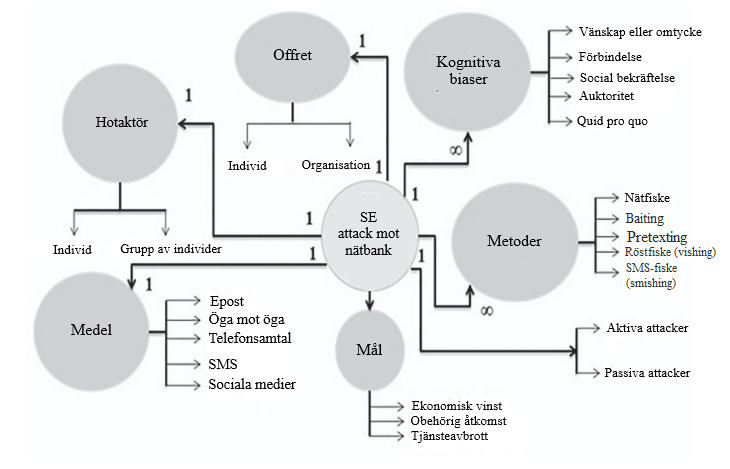
\includegraphics[width=\textwidth]{Bilder/SE33}
    \caption{En översättning av bilden \textit{Ontology model of social engineering in e-banking} \cite{gururaj2024social_engineering}.}
    \label{fig:se_samhällskritiska}
\end{figure}

För att motverka social engineering inom samhällskritiska system använder många organisationer avancerade tekniska skyddsåtgärder, såsom flerfaktorautentisering (MFA), nätverkssegmentering och intrångsdetektionssystem. Oavsett dessa avancerade system fortsätter den mänskliga faktorn inom systemen att utgöra en betydande sårbarhet \cite{washo2021interdisciplinary, albladi2018defense_mechanisms}. Särskilt utsatta är operativa gränssnitt där mänskligt beslutsfattande kombineras med tekniska processer, såsom helpdesk-funktioner, administrativ åtkomsthantering och leverantörskommunikation. Som tidigare betonats av \cite{washo2021interdisciplinary, enisa2018cybersecurity_culture} påverkar organisatoriska strukturer och arbetsprocesser hur motståndskraftiga dessa gränssnitt är mot manipulation. 

\section{Fallstudier av social engineering-relaterade incidenter}
För att förtydliga hur social engineering framträder i praktiken analyseras i detta avsnitt utvalda verkliga incidenter. Fallstudierna syftar till att illustrera hur social engineering kan användas för både ekonomisk vinning och strategisk samhällspåverkan. Angreppsmetoder som tidigare presenterats kommer också att behandlas, där attackerna tillämpas i organisatoriska och politiska sammanhang. Fallstudierna kommer också att illustrera hur avancerade tekniska verktyg, som AI, kan förstärka manipulationens effektivitet.

\subsection{Arup djupfejk-bedrägeri}
Under 2024 utsattes det internationella teknikkonsultföretaget Arup för en omfattande social engineering-attack där AI användes för att genomföra ett avancerat djupfejk-bedrägeri \cite{guardian_arup_2024, bbc_arup_2024}. Händelsen lyfte fram hur AI i moderna social engineering-attacker kan förstärka traditionella manipulationsmetoder och skapa nya säkerhetsutmaningar för organisationer.

En anställd vid företagets kontor i Hongkong mottog ett meddelande som påstods komma från företagets ekonomichef (CFO). Kort därefter deltog den anställde i ett videomöte där flera personer som såg ut och lät som företagets chefer deltog. Enligt rapportering från både BBC och The Guardian var samtliga deltagare i videomötet AI-genererade djupfejkar, där hotaktörerna hade manipulerat både bild och ljud för att imitera verkliga personer inom organisationen \cite{guardian_arup_2024, bbc_arup_2024}. Under mötet anvisades den anställde att genomföra ett antal banköverföringar till olika konton. Totalt överfördes cirka 20-25 miljoner amerikanska dollar genom flera separata transaktioner innan bedrägeriet upptäcktes \cite{guardian_arup_2024, bbc_arup_2024}. Arup bekräftade senare incidenten och att den utgjorde en form av teknologiskt förstärkt bedrägeri.

Ur ett cybersäkerhetsperspektiv visar Arup-fallet hur social engineering kan utvecklas genom integration av AI. Attacken byggde inte endast på utnyttjandet av tekniska sårbarheter i nätverk eller system, utan också på manipulation av en anställds förtroende i en situation som framstod som legitim \cite{algarni2019se_survey}. Denna specifika incident överensstämmer med tidigare forskning från \cite{algarni2019se_survey} där social engineering påstås fungera som en intrångsvektor, där hotaktören utnyttjar mänskligt beslutsfattande istället för tekniska brister.  

Vidare hänvisar incidenten till utvecklingen av AI-stödd social engineering, där generativa modeller används för att producera språkligt och visuellt övertygande innehåll \cite{zhang2024digital_deception}. Genom att kombinera djupfejkteknik med organisatorisk kontext skapade hotaktörerna ett trovärdigt scenario där traditionella tekniska säkerhetsåtgärder inte räckte till. Fallet bekräftar även \cite{algarni2024comprehensive_taxonomy} där det observeras att moderna social engineering-attacker ofta kombinerar tekniska och sociala komponenter i en integrerad angreppsstrategi. Djupfejk-elementet utgjorde den tekniska komponenten, medan manipulationen av organisatoriska rutiner och beslutsprocesser utgjorde den sociala. Kombinationen möjliggjorde ett intrång utan att hotaktörerna behövde bryta igenom tekniska skyddssystem.  

\subsection{USA:s presidentval 2016}
Förutom ekonomiskt motiverade attacker har social engineering också använts för politiska ändamål. Enligt \cite{fiia2016election_hacking} har flera demokratiska val blivit utsatta för koordinerade cyber- och desinformationsoperationer där teknik och psykologisk manipulation har kombinerats för att kontrollera informationsflödet. En av de mest dokumenterade exemplen på hur social engineering kan användas inom demokratiska val är USA:s presidentval 2016.

Under valrörelsen genomfördes riktade spjutfiske-attacker mot politiska kampanjorganisationer, som exempelvis Democratic National Committee (DNC). Genom nätfiskeattacker som utgav sig för att vara legitima säkerhetsvarningar lyckades hotaktörerna få tillgång till interna e-postkonton. Efter det lyckade intrånget började den stulna kommunikationen att publiceras via externa plattformar. Enligt \cite{fiia2016election_hacking} användes den stulna informationen strategiskt för att skapa uppmärksamhet på sociala medier och orsaka politisk polarisering och misstro. Syftet med attacken var därmed inte att manipulera rösträkningen rent tekniskt, utan att påverka det informationsmässiga och psykologiska klimatet kring valet. Enligt internationella utredningar kopplades attackerna i ett senare skede till statligt associerade ryska aktörer, vilket placerade incidenten i ett bredare geopolitiskt sammanhang \cite{fiia2016election_hacking}.

Fallstudiet kan ses ur ett cybersäkerhetsperspektiv som en kombination av spjutfiske och desinformationsmanipulation. Angreppets initiala fas riktade sig mot enskilda individer genom social engineering, medan senare faser syftade till en samhällelig påverkan. Här blir kopplingen till en bredare definition av social engineering tydlig. Som tidigare nämnts beskriver \cite{podgorecki1998social} social engineering som ett försök att medvetet forma sociala strukturer och kollektiva beteenden genom strategisk påverkan. I fallet med USA:s presidentval 2016 riktades attacken inte mot enskilda individer, utan mot röstare och det demokratiska förtroendet som helhet. Här betonas samma princip av \cite{fiia2016election_hacking} att, även om den tekniska valinfrastrukturen inte nödvändigtvis manipulerades direkt, kunde desinformationsoperationerna påverka hur valet uppfattades.



\section{Konsekvenser av social engineering-attacker}
Som diskuterats ovan kan social engineering medföra konsekvenser som sträcker sig långt bortom från det initiala intrånget. Beroende på kontext kan effekterna vara ekonomiska, organisatoriska, politiska eller samhälleliga. Oberoende av motivationen bakom attacken har dessa alla gemensamt att de uppstår genom manipulation av mänskligt beslutsfattande snarare än direkt tekniskt utnyttjande. 

Ur ett ekonomiskt perspektiv kan social engineering leda till allvarliga finansiella förluster. Arup-incidenten visar hur manipulation av en enskild anställd möjliggjorde överföring av miljontals amerikanska dollar utan att tekniska säkerhetssystem bröts \cite{bbc_arup_2024, guardian_arup_2024}. Liknande incidenter för med sig inte endast direkta ekonomiska förluster, utan även sekundära konsekvenser, såsom rättsliga utredningar, sanktioner och ökade säkerhetsinvesteringar. I organisatoriska sammanhang kan social engineering påverka förtroendet inom och mellan organisationer. När autentiseringsprocesser manipuleras, eller kommunikationskanaler utnyttjas, kan detta skapa osäkerhet kring rutiner och misstro mellan anställda. Enligt ENISA är säkerhetskultur och tydliga processer avgörande för att minska denna typ av organisatorisk sårbarhet \cite{enisa2018cybersecurity_culture}. Efter en incident kan organisationer tvingas att omvärdera sina säkerhetsstrategier och införa striktare kontroller, vilket kan leda till försämrad effektivitet och arbetsflöde. 

På en samhällelig nivå kan konsekvenserna vara mer omfattande. USA:s presidentval 2016 illustrerar hur social engineering kan användas för att påverka informationsmiljöer och skapa skepticism \cite{fiia2016election_hacking}. Användningen av nätfiske och informationsmanipulering bidrog till ökad polarisering och misstro kring valet. Som incidenten klart visar, var målet med attacken inte att nå ekonomisk vinst, utan att påverka kollektiv perception och politiskt förtroende. 

\begin{figure}[H]
    \centering
    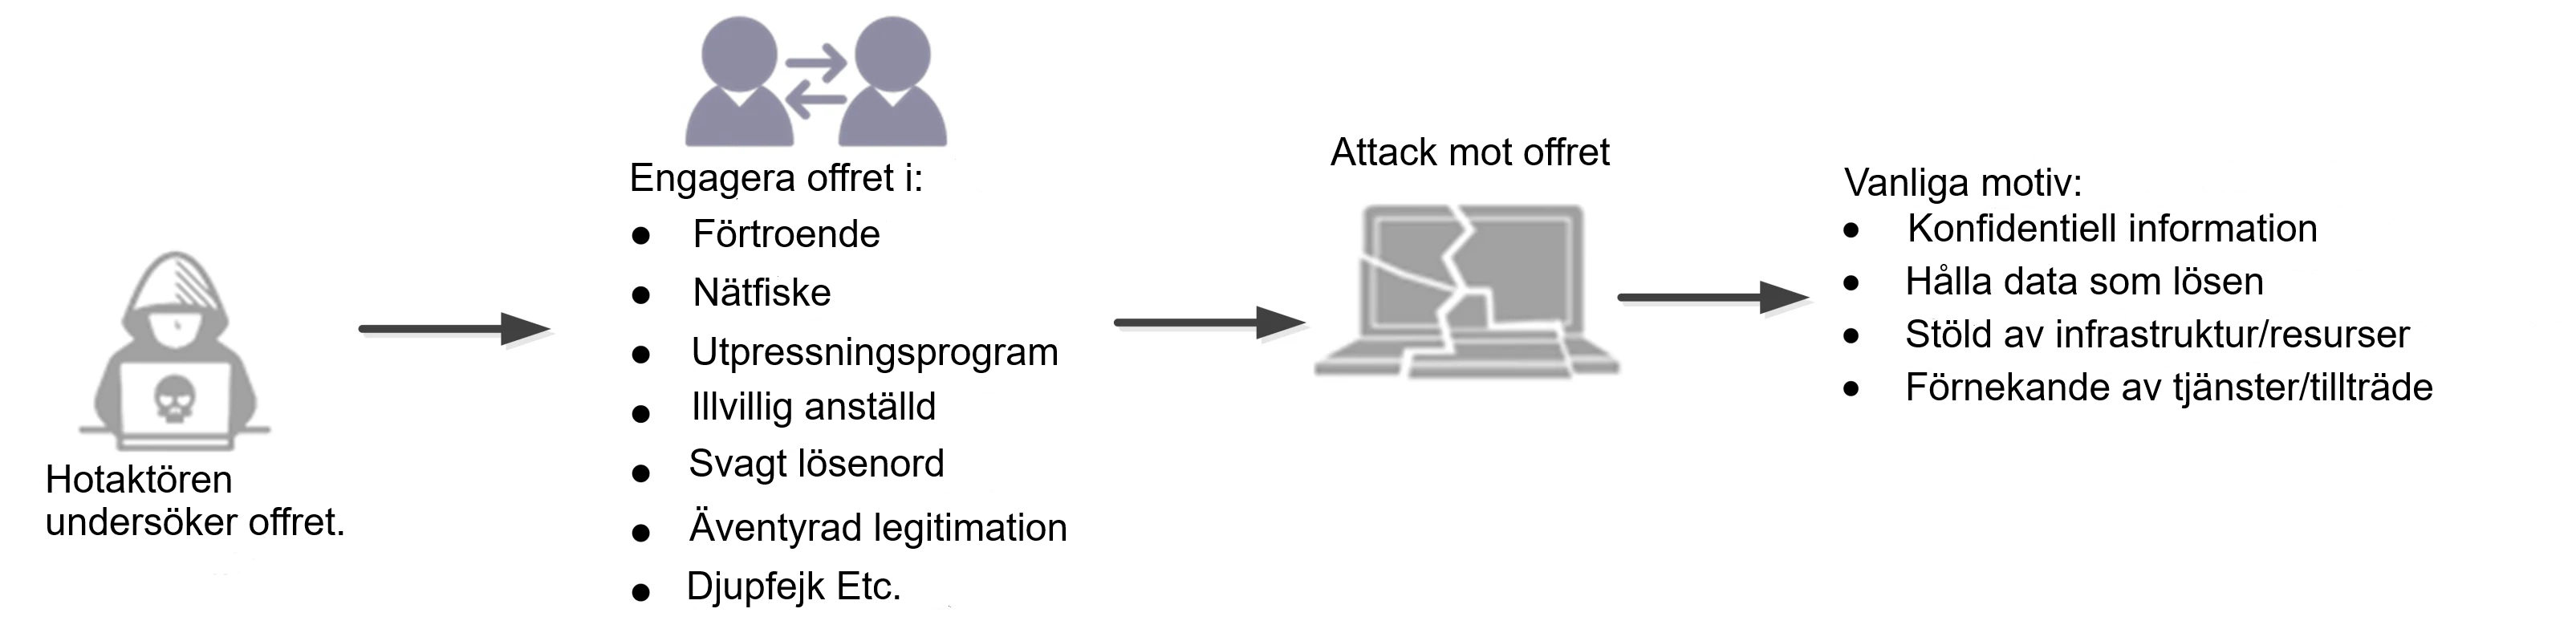
\includegraphics[width=\textwidth]{Bilder/A Study on the Psychology}
    \caption{En översättning av bilden \textit{A basic flow of social engineering-based cyberattacks} \cite{psychology_social_engineering}.}
    \label{fig:se_Konsekvenser}
\end{figure}

Från ett psykologiskt perspektiv påverkar social engineering-attacker också individers säkerhetsbeteende. Enligt \cite{psychology_social_engineering} kan manipulationen genom brådska, auktoritet och stress leda till att individer underskattar risker eller agerar impulsivt. Efter en social engineering-incident kan individers säkerhetsbeteenden förändras på olika sätt. I vanliga fall leder händelsen till ökad vaksamhet, där användare blir mer försiktiga och uppmärksamma. I andra fall kan däremot upprepade varningar, säkerhetsförfrågningar och autentiseringsmeddelanden skapa så kallad säkerhetsutmattning \cite{albladi2019training_awareness}. Fenomenet innebär att individer, på grund av stress eller vana, börjar ignorera varningar eller godkänna förfrågningar utan noggrann observation. 

Slutligen bidrar upprepade social engineering-incidenter även till en förskjutning i hotlandskapet. Enligt \cite{aldawood2019taxonomy, algarni2019se_survey, algarni2024comprehensive_taxonomy} utvecklas angreppsmetoder kontinuerligt genom tekniska verktyg och social manipulation. Detta innebär att konsekvenserna är reaktiva och att organisationer och samhällen måste konstant anpassa sig för att hantera cyberhotet. 

\chapter{Tekniska motåtgärder mot social engineering}
Kapitlet kommer att analysera tekniska motåtgärder som kan användas för att förebygga, identifiera och begränsa social engineering-attacker. 
Som stöd används de angreppsmetoder och fallstudier som tidigare presenterats där en analys av hur tekniska säkerhetsåtgärder kan förstärka motståndskraften mot 
social manipulation. Inledningsvis diskuteras metoder för identifiering och detektion av social engineering-relaterade attacker. Därefter behandlas artificiell 
intelligens som en potentiell försvarsmekanism, med fokus på dess effektivitet och begränsningar. Avslutningsvis diskuteras autentisering och åtkomstkontroll som 
tyngdpunkt i skyddet mot obehörig åtkomst och identitetsbedrägeri.

\section{Identifiering och detektion av social engineering-attacker}
Eftersom social engineering riktar sig mot mänskligt beslutsfattande kan identifiering av dessa attacker vara särskilt svår. Till skillnad från traditionella intrång, 
där skadlig kod eller nätverksintrång kan upptäckas genom teknisk övervakning, sker social manipulation ofta genom kommunikationskanaler som e-post, 
short message service (sms) eller sociala medier \cite{se_threat_defense_survey, algarni2019se_survey}. Av denna anledning fokuserar en stor del av detektionsarbetet 
på tekniska filtrerings- och analysmekanismer. I nätfiskedetektion används exempelvis e-postfiltrering samt analys av URL-strukturer, domänvalidering och 
maskininlärningsbaserade klassificeringsmodeller för att identifiera suspekta meddelanden innan de når offret \cite{basnet2023anti_phishing}. Systemen kan exempelvis 
analysera avsändarinformation, språkmönster och beteendeavvikelser för att markera potentiellt skadligt innehåll.

Utöver de ovannämnda detektionssystemen används ofta säkerhetsinformation och händelsehantering (SIEM-system) för att samla in och korrelera säkerhetsloggar från olika 
delar av en organisations infrastruktur. Genom kombinationen av SIEM och intrångsdetekteringssystem (IDS) kan misstänkt aktivitet identifieras i realtid. 
Enligt \cite{siem_comprehensive_study_2022} visar integrationen av SIEM och IDS med maskininlärningsmodeller en förbättrad förmåga att upptäcka ovanliga inloggningar 
eller typiska åtkomstförsök. Moderna organisationer har även börjat implementera Security Orchestration, Automation and Response (SOAR-system). Ett SOAR-system integrerar 
flera olika säkerhetsverktyg i en gemensam miljö som möjliggör automatiserad hantering av säkerhetsincidenter \cite{almohri2024soar}. Genom insamlade data från exempelvis 
SIEM-system, e-postfilter och hotinformationsdatabaser kan SOAR automatiskt initiera åtgärder såsom blockering av konton, isolering av enheter eller återkallande av 
skadliga länkar. Därmed möjliggör SOAR snabbare identifiering och respons vid social engineering-relaterade incidenter.

Trots alla dessa system kvarstår utmaningar. Eftersom social engineering bygger på psykologi snarare än teknik, kan välkonstruerade attacker fortfarande undvika 
traditionella säkerhetsfilter \cite{algarni2019se_survey}. Därför betonas i organisatoriska sammanhang vikten av att kombinera tekniska detektionssystem med 
organisatoriska rutiner och användarmedvetenhet för att uppnå optimalt skydd.

\section{Artificiell intelligens som försvarsmekanism}
Utvecklingen av AI har dragit med sig både för- och nackdelar inom cybersäkerhet. I dagens cyberhotlandskap har AI sett en ökad användning av hotaktörer för att 
exempelvis skapa mer övertygande nätfiskeattacker eller djupfejkmaterial, medan samma teknologi har blivit ett centralt verktyg för att motverka dessa social 
engineering-attacker \cite{zhang2024digital_deception}.

Orsaken till att AI har blivit ett viktigt verktyg för att motverka social engineering-attacker är dess förmåga att analysera stora kvantiteter av data och identifiera mönster 
som kan vara svåra att upptäcka manuellt. I nätfiskedetektion används exempelvis maskininlärningsmodeller för att enkelt markera e-postmeddelanden baserat på språk, 
metadata, URL-strukturer och avsändarbeteende \cite{basnet2023anti_phishing}. Genom att kontinuerligt träna modellerna med nya data kan försvaret mot social engineering 
upprätthållas i realtid. Enligt \cite{zhang2024digital_deception, basnet2023anti_phishing} kan AI även användas för att förstärka användarstöd och beslutsfattande. Genom specialiserade varningssystem 
och kontextbaserade säkerhetsindikatorer kan AI minska risken för impulsivt agerande vid en social engineering-attack. 

Som redan nämnt fungerar AI inte endast som en universallösning. Eftersom hotaktörer också använder AI för att skapa mer sofistikerade angrepp, uppstår det en form av kapprustning \cite{zhang2024digital_deception}. 
För att hållas i kapp måste därför försvarssystem kontinuerligt uppdateras och kombineras med organisatoriska säkerhetsrutiner \cite{algarni2024comprehensive_taxonomy}.



\subsection{Användningen av maskininlärning för detektion}
Som nämnts ovan utgör maskininlärning (ML) en central del av AI-baserade försvarssystem mot social engineering. Till skillnad från traditionella försvarssystem, som kräver fördefinierade kriterier, 
kan användningen av övervakad och oövervakad maskininlärning användas för att identifiera komplexa mönster även i stora datamängder \cite{basnet2023anti_phishing}. 
Användningen av metoderna möjliggör anpassning till kontinuerligt förändrande attacker.

I nätfiske-relaterad detektion används ofta övervakad inlärning, där modeller tränas på specifika dataset bestående av skadliga och ofarliga meddelanden. Genom att fokusera på exempelvis 
analys av språkliga strukturer, avsändardomäner, metadata och förekomsten av språkliga indikatorer på brådska, såsom tidsbegränsningar, krav på omedelbar åtgärd eller hot om negativa konsekvenser, 
kan modellen klassificera nya meddelanden med större sannolikhet \cite{basnet2023anti_phishing}. Metoden möjliggör konstant förbättring av detektionsprecisionen i takt med nya data. Utöver övervakad 
inlärning används också oövervakad inlärning för att identifiera avvikande beteendemönster. I dessa fall analyseras en användares aktivitetsmönster, som exempelvis inloggningstider och geografisk placering. 
Om användarens beteende avviker i stor grad från det normala kan systemet generera en varning om ett potentiellt äventyrande konto \cite{siem_comprehensive_study_2022}. Metoden är därför särskilt användbar i 
situationer där hotaktören redan har fått åtkomst till autentiseringsuppgifter genom lyckad social engineering.  

ML används även i kombination med SIEM- och IDS-system för att möjliggöra realtidsanalys av nätverkstrafik och autentiseringsloggar \cite{siem_comprehensive_study_2022}. Genom att använda flera datakällor 
kan systemet skapa en helhetsbild av det potentiella hotet. Integrationen möjliggör förbättrad identifiering av komplexa attacker som kombinerar tekniskt utnyttjande med social manipulation. Oavsett sina styrkor 
har ML också begränsningar. Modellerna är mycket beroende av kvaliteten på träningsdata och kan vara särskilt känsliga för så kallade fientliga attacker, där hotaktörer medvetet manipulerar inputdata för att undvika 
detektion \cite{algarni2024comprehensive_taxonomy}. ML bör därför förstås som en del av en helhetsstrategi istället för en självständig lösning.

\subsection{Begränsningar och risker med AI}
Även om AI erbjuder avancerade möjligheter för detektion och respons med hjälp av ML, är teknologin ingen universallösning mot social engineering. Eftersom ML utgör en central del av många AI-baserade system påverkas AI 
indirekt av samma begränsningar som ML-modeller uppvisar, såsom beroende av träningsdata, modellarkitektur och kontinuerliga uppdateringar \cite{basnet2023anti_phishing, algarni2024comprehensive_taxonomy}. Om träningsdata är bristfälliga eller utsätts för en fientlig attack, kan modellen utveckla brister i 
sin klassificeringsförmåga. Därtill kvarstår det centrala problemet med AI, vilket är att hotaktörerna också använder sig av AI. Användningen av AI 
skapar då indirekt en osynlig teknologisk kapprustning där både angripare och försvarare använder sig av samma verktyg för att ligga steget före den andra \cite{zhang2024digital_deception}.

Dessutom förekommer det fler begränsningar med AI i form av dess analyseringsprocesser. AI analyserar tekniska indikatorer, medan social engineering i grunden är ett socio-tekniskt fenomen \cite{washo2021interdisciplinary}. 
Manipulationer sker i mänskliga sammanhang, organisatoriska rutiner och beslutsprocesser, där även de mest avancerade AI-systemen inte fullt kan ersätta mänskligt beslutsfattande eller  säkerhetskultur. Därpå kan nya risker 
uppstå i organisationer på grund av ett överdrivet beroende av AI. Överdrivet beroende kan leda till utvecklingen av falsk trygghet och förlitande på AI-baserat skydd, vilket därmed kan leda till minskad vaksamhet eller riskbedömning.  

\section{Autentisering och åtkomstkontroll}
Eftersom social engineering är en kombination av både psykologisk manipulation och användning av tekniska verktyg, krävs det mer avancerade lösningar för att uppnå optimalt skydd. Tekniska system, som AI-baserat skydd, 
kan identifiera och blockera många sorters angrepp, men den mänskliga faktorn kvarstår i beslutsprocesser och beteendemönster. Specifikt när det gäller organisationer spelar säkerhetskultur, utbildningsnivå och interna rutiner en avgörande 
roll i hur motståndskraftiga de är mot social engineering \cite{washo2021interdisciplinary}. Trots de olika motåtgärderna är utbildnings- och medvetandeprogram riktade till anställda bland de mest använda säkerhetsåtgärdererna. Enligt \cite{albladi2019training_awareness} är 
dessa utbildningsprogram dock bristfälliga, eftersom utbildningen ofta erbjuds endast några gånger istället för kontinuerligt. För att uppnå ett effektivt skydd bör utbildningen vara återkommande, scenariobaserad och anpassad 
efter organisationens behov. 

ENISA betonar betydelsen av att utveckla en stark cybersäkerhetskultur där säkerhetsbeteenden integreras i vardagliga rutiner \cite{enisa2018cybersecurity_culture}. Integrationen av cybersäkerhetskultur innebär att säkerheten 
inte endast ska fungera som en teknisk funktion utan även som en del av organisationen och dess ledarskap. När dessa säkerhetsprinciper tydligt är anpassade till organisationens struktur minskar sannolikheten för lyckad manipulation. 
Ett exempel på detta är användningen av simulerade nätfiskekampanjer för att mäta och förbättra arbetarnas motståndskraft \cite{albladi2018defense_mechanisms}. Genom kontrollerade tester kan organisationer identifiera sårbarheter och 
anpassa utbildningsinsatser baserat på resultaten. Samtidigt måste även dessa simuleringar genomföras med hänsyn till organisatorisk tillit och arbetsmiljö, eftersom övervakning kan påverka arbetarnas upplevelse och trygghet.

Utöver olika utbildningar är tydliga policyer och rutiner viktiga för säkerheten \cite{gururaj2024social_engineering}. Principer som lägsta behörighet, tydliga verifieringsprocesser vid ekonomiska transaktioner och 
användning av flerfaktorautentisering bidrar också till förbättrat skydd \cite{algarni2024comprehensive_taxonomy}. Genom att implementera dessa strukturella säkerhetsåtgärder kan organisationer begränsa skadan även om en 
individ blir utsatt för manipulation.

\chapter{Diskussion}

Social engineering som ett cyberhot har bevisats utmana uppdelningen mellan teknisk och mänsklig säkerhet.
Medan traditionella cybersäkerhetsmodeller ofta fokuserar på systemarkitektur, nätverksskydd och tekniska sårbarheter,
utnyttjar social engineering i första hand organisatoriska strukturer och mänskliga beslutsprocesser.
Detta innebär att angreppsytan för social engineering-relaterade attacker inte endast utgörs av tekniska system som servrar,
protokoll eller autentiseringssystem, utan även av arbetsrutiner, hierarkier och sociala relationer. I motsats till rent tekniska attacker, där sårbarheter ofta kan identifieras och åtgärdas,
är den mänskliga faktorn i social engineering-attacker mer dynamisk och svår att standardisera. En organisation
kan implementera flerfaktorautentisering (M2FA), SOAR-system och AI-baserad detektion, men om en anställd ändå blir manipulerad av en hotaktör
att lämna ut känsliga data eller utföra en skadlig handling, förlorar systemen sin effektivitet. För organisationer betyder detta
att säkerhetsnivån är beroende av både tekniska kontroller och mänskligt omdöme, där den svagaste länken kan avgöra utfallet.

Utvecklingen av AI har endast förstärkt problemet. Medan AI möjliggör mer avancerad detektion och analys, har samma teknologi också börjat användas av hotaktörer
för att skapa mer avancerade attacker, som djupfejk-baserade bedrägerier. Resultatet leder till en teknologisk symmetri där försvar och angrepp utvecklas pararellt. 
Här uppstår det frågan om avancerad teknik kan lösa problemet, eller om den endast förändrar dess form. Organisatorisk säkerhetskultur kopplar sig också till problemet.
I teorin kan säkerhetsutbildning och medvetandeprogram minska risken för lyckad manipulation. I praktiken orsakar överexponering för varningar och säkerhetsrutiner säkerhetsutmattning,
där anställda rutinmässigt godkänner förfrågningar utan noggrann granskning. Detta illusterar att även välmenade säkerhetsåtgärder kan orsaka motsatt effekt om de inte balanseras med 
användarbarhet och organisatoriska rutiner.

Social engineering tar fram också en bredare fråga om ansvarsfördelning. Om en attack lyckas genom manipulation av en individ, ligger ansvaret på den enskilda användaren,
organisationens rutiner eller systemdesignen? Oftast kritiseras den ``bristfälliga användaren``, men forskning har visat att säkerhetsdiskurser ibland individualiserar problemet,
medan sårbarheten ofta är strukturell. Därför måste det tas hänsyn till att social engineering-relaterade incidenter är ett symptom på organisatoriska och kommunikativa brister,
snarare än enbart individuella misstag. Fallstudierna visar därutöver att konsekvenserna varierar i stor grad beroende på kontext. I ekonomiskt motiverade attacker är målet direkt
finansiell vinning, medan politiskt motiverade attacker syftar till att påverka samhälleligt förtroende och informationsmiljöer. Variationen bakom motivet av attacken indikerar att
social engineering inte är en homogen angreppsform utan en flexibel metod som anpassas efter målsättning. 

\chapter{Slutsats}

Social engineering har i denna avhandling analyserats som ett cybersäkerhetshot med fokus på samverkan mellan psykologiska och tekniska aspekter av digital manipulation.
Den första forskningsfrågan har besvarats genom att analysera hur social engineering bygger på systematiska kognitiva biaser och sociala principer såsom auktoritet, brådska,
tillit och social bekräftelse. Dessa psykologiska mekanismer påverkar individers beslutsfattande och minskar benägenheten att kritiskt granska situationer som framstår som legitima.
Angreppens effektivitet ligger därmed inte endast i teknisk komplexitet, utan också i förmågan att manipulera mänskliga beteendemönster och organisatoriska normer.

Den andra forskningsfrågan har besvarats med att visa hur moderna social engineering-attacker ofta kombinerar traditionella metoder såsom nätfiske, spjutfiske, pretexting, baiting 
och insider-relaterade attacker med tekniska komponenter som artificiell intelligens, domänförfalskning och automatiserade meddelandesystem. Fallstudierna illustrerar även hur
AI-baserade djupfejkar och riktade informationsoperationer ytterligare förstärker attackernas trovärdighet och effektivitet. Social engineering-attacker visar därmed hur
flexibla och anpassningsbara de är, då både tekniska och sociala element kombineras för en unik angreppsstrategi.

Den tredje forskningsfrågan har besvarats genom att analysera olika detektionssystem som främst bygger på tekniska filtreringssystem, maskininlärningsbaserad analys, SIEM- och IDS-integration
samt automatiserade responsmekanismer såsom SOAR. Dessa system kan upptäcka avvikande beteenden, misstänkt kommunikation och ovanliga åtkomstförsök. Det visades också att systemen
måste kompletteras med organisatoriska rutiner och säkerhetskultur, eftersom manipulationen ofta riktas mot mänskligt beslutsfattande snarare än enbart tekniska sårbarheter.

Den fjärde forskningsfrågan har besvarats genom att analysera den artificiella intelligensens potential inom detektion och respons genom avancerad mönsterigenkänning och beteendeanalys.
AI kan bidra till snabbare identifiering av cyberhot och effektivare hantering av incidenter. Däremot begränsas samtidigt teknologins effektivitet av faktorer som datakvalitet, falska resultat och
det faktum att hotaktörer också använder AI för att förbättra sina angreppsstrategier. AI bör därför förstås som en relevant del av försvarsstrategier mot social engineering, men inte
som en självständig lösning.
 

\clearpage
\chapter*{Källförteckning}
\addcontentsline{toc}{chapter}{Källförteckning}

\nocite{*} % ta bort senare när du citerar i texten
\printbibliography[heading=none]

\end{document}